\chapter{Decomposição Adaptativa}
\label{chap:decomposicao-adaptativa-clustering}

Como descrito anteriormente, cada par entidade-núcleo é representado por uma 
variável binária. Para $N$ entidades e $K$ núcleos, o número de qubits lógicos 
necessários é:

\begin{equation}
    n_q = N \cdot K.
\end{equation}
\listeq{Número de qubits necessários sem decomposição}

Como $n_q$ cresce linearmente com $N$, instâncias com muitas entidades rapidamente
excedem os limites práticos de escala do hardware quântico atual, marcado por baixa contagem
de qubits e elevadas taxas de erro ~\cite{Preskill2018}. Por exemplo, para $K=8$ núcleos e $N=50$ entidades,
são necessários $n_q = 400$ qubits, um valor que já excede a capacidade da maioria dos
dispositivos atuais.

Para contornar esta limitação, a plataforma 
inclui uma etapa de decomposição adaptativa: em vez de considerar todas as entidades 
em simultâneo, estas são agrupadas em conjuntos de menor dimensão, 
designados \textit{bundles}, formados com base na semelhança entre processos, considerando a sua carga de CPU e memória usada. 

Esta abordagem vem que o QAOA opera sobre entidades e as suas cargas agregadas, sem distinguir se cada entidade corresponde a um processo isolado ou a um grupo de procesos, basta que os processos dentro do mesmo bundle sejam suficientemente homogéneos em carga que o bundle comporta-se como uma entidade equivalente e a qualidade da solução não é degradada.

A afinidade de memória complementa a decomposição para evitar juntar processos com perfis de memória muito diferentes.

Considere-se um \textit{snapshot} com um conjunto de processos
$\mathcal{P} = \{p_1, p_2, \dots, p_N\}$ e $K$ núcleos disponíveis. Em primeiro lugar, os processos de tempo real são separados dos restantes, definindo-se $\mathcal{P}_{N} = \mathcal{P} \setminus \mathcal{P}_{RT}$.

Os processos em $\mathcal{P}_{RT}$ mantêm a sua atribuição fixa ao núcleo atual, 
uma vez que processos de tempo real têm requisitos de latência estritos que 
desaconselham a sua reatribuição. A decomposição adaptativa é aplicada apenas aos processos normais $\mathcal{P}_{N}$.

Dado um limite máximo de qubits $q_{max}$, define-se o número máximo de processos representáveis por \textit{bundle} como:

\begin{equation}
    m = \left\lfloor \frac{q_{max}}{K} \right\rfloor.
\end{equation}
\listeq{Número máximo de processos por bundle}

Para $N_N = |\mathcal{P}_{N}|$ processos normais, o número inicial de \textit{bundles} é calculado por:

\begin{equation}
    B = \min\left(
        \left\lceil \frac{N_N}{m} \right\rceil,
        N_N
    \right).
\end{equation}
\listeq{Número adaptativo de bundles}

Quando $B \geq N_N$, não é necessário agrupar processos, pelo que cada processo é
representado por um \textit{bundle} individual.

Caso contrário, os processos são
agrupados recorrendo a \textit{spectral clustering}~\cite{Ng2001Spectral}. Ao contrário
de métodos como o K-Means, que tendem a formar grupos de tamanho semelhante e forma
regular, o \textit{spectral clustering} consegue detetar agrupamentos naturais nos
dados mesmo quando estes têm formas irregulares --- uma propriedade relevante em
\textit{snapshots} reais, onde os processos podem formar grupos de diferentes tamanhos
e densidades. Para isso, é necessário primeiro construir uma matriz de afinidade entre
processos.


Para cada processo $p_i$, começa-se por calcular uma carga efetiva de \acs{CPU}, reduzindo o peso de processos que passam parte significativa do tempo em espera por \textit{I/O}:

\begin{equation}
    \tilde{w}_i =
    w_i \left(1 - \alpha_{io} r_i \right),
\end{equation}
\listeq{Carga efetiva de CPU}

onde $w_i$ representa a carga de \acs{CPU} observada, $r_i \in [0,1]$ é a fração de tempo em espera por \textit{I/O}, e $\alpha_{io}$ controla o impacto dessa espera na carga efetiva.

Esta correção é relevante porque melhora a qualidade da informação usada para
construir a matriz de afinidade entre processos: ao distinguir processos
\emph{CPU-bound} de processos \emph{I/O-bound}, permite que a decomposição
agrupe processos com perfis semelhantes de forma mais precisa, melhorando a
qualidade da decomposição.

Cada processo é então representado por um vetor de características com duas componentes:

\begin{equation}
    \mathbf{f}_i =
    \begin{bmatrix}
        \tilde{w}_i \\
        \mathrm{rss}_i
    \end{bmatrix},
\end{equation}
\listeq{Vetor de características de um processo}

onde $\mathrm{rss}_i$ corresponde à memória residente do processo.

Com base nas características de cada processo, é construída uma matriz de afinidade $A$, que mede a semelhança entre pares de processos. O objetivo é agrupar processos com perfis semelhantes --- por exemplo, processos com pouca utilização de \acs{CPU} e elevada utilização de memória devem ficar no mesmo \textit{bundle}.
Para isso, são consideradas duas componentes: utilização de \acs{CPU} e memória (a utilização de I/O também é aplicada indiretamente através do peso efetivo $\tilde{w}_i$).
A distância
entre dois processos em cada componente é medida pelo quadrado da diferença dos
valores normalizados:

\begin{equation}
    d^{cpu}_{ij} = \left(\hat{f}_{i,cpu} - \hat{f}_{j,cpu}\right)^2,
    \qquad
    d^{mem}_{ij} = \left(\hat{f}_{i,mem} - \hat{f}_{j,mem}\right)^2.
\end{equation}
\listeq{Distâncias quadráticas nas componentes CPU e memória}

Distâncias menores indicam processos mais semelhantes. No entanto, o \emph{spectral clustering} opera sobre afinidades, não sobre distâncias: valores altos devem indicar processos semelhantes, e não o contrário. Para converter estas
distâncias em afinidades, aplica-se um kernel RBF, fazendo com que a afinidade decresça rapidamente à medida que os processos se tornam mais distintos:

\begin{equation}
    A^{cpu}_{ij} = \exp\left(-\frac{d^{cpu}_{ij}}{2\sigma_{cpu}^{2}}\right),
    \qquad
    A^{mem}_{ij} = \exp\left(-\frac{d^{mem}_{ij}}{2\sigma_{mem}^{2}}\right).
\end{equation}
\listeq{Afinidades RBF para CPU e memória}

Os parâmetros $\sigma_{cpu}$ e $\sigma_{mem}$ são calculados como a mediana
das distâncias entre todos os pares de processos.

A matriz de afinidade final combina as duas componentes:

\begin{equation}
    A_{ij} = \alpha A^{cpu}_{ij} + (1-\alpha) A^{mem}_{ij}, \qquad i \neq j,
\end{equation}
\listeq{Matriz de afinidade combinada}
O parâmetro $\alpha$ controla a 
importância relativa da utilização de \acs{CPU} face à utilização de memória.

O algoritmo devolve uma função de atribuição:
\begin{equation}
    g : \mathcal{P}_{N} \rightarrow \{0, 1, \dots, B-1\},
\end{equation}
\listeq{Atribuição de processos a bundles}

onde $g(p_i)$ indica o \textit{bundle} atribuído ao processo $p_i$. Para cada 
\textit{bundle} $b$, são calculadas as grandezas agregadas de \acs{CPU} e memória:

\begin{equation}
    W_b = \sum_{p_i : g(p_i)=b} \tilde{w}_i,
    \qquad
    R_b = \sum_{p_i : g(p_i)=b} \mathrm{rss}_i.
\end{equation}
\listeq{Carga de CPU e memória agregadas por bundle}

Cada \textit{bundle} passa então a ser tratado como uma única entidade na 
formulação \acs{QUBO}, com peso $W_b$ e memória agregada $R_b$.


\subsection{Verificações de Qualidade e Divisão Recursiva}

O clustering inicial pode produzir \textit{bundles} problemáticos: um bundle pode
ser internamente heterogéneo, ou concentrar carga excessiva de \acs{CPU} ou memória. Em qualquer destes casos, representá-lo como uma 
única entidade no \acs{QUBO} introduziria imprecisão na formulação. Por isso, após 
o clustering inicial, cada \textit{bundle} é sujeito a três verificações:

\begin{itemize}
    \item \textbf{Heterogeneidade interna}: medida pelo coeficiente de variação da carga dos processos no bundle,
    \begin{equation}
        CV_b = \frac{\operatorname{std}\left(\{\tilde{w}_i : g(p_i)=b\}\right)}
                    {\operatorname{mean}\left(\{\tilde{w}_i : g(p_i)=b\}\right)}.
    \end{equation}
    \listeq{Coeficiente de variação de um bundle}
    Um bundle é considerado heterogéneo quando $CV_b$ excede um limiar configurável.

    \item \textbf{Peso outlier}: a carga agregada $W_b$ é comparada com a 
    distribuição dos restantes \textit{bundles} através do z-score,
    \begin{equation}
        z_b = \frac{W_b - \mu_W}{\sigma_W},
    \end{equation}
    \listeq{Z-score da carga agregada de um bundle}
    onde $\mu_W$ e $\sigma_W$ são a média e o desvio padrão das cargas agregadas. 
    Um bundle é considerado demasiado pesado quando $|z_b|$ excede um limiar 
    configurável.

    \item \textbf{Pressão de memória}: a memória agregada $R_b$ é comparada com 
    um limiar configurável.
\end{itemize}

Se um \textit{bundle} falhar pelo menos uma destas verificações e contiver mais do 
que um processo, é dividido em dois sub-bundles usando K-Means sobre os pesos 
efetivos de \acs{CPU}. Cada sub-bundle é depois avaliado recursivamente com as 
mesmas verificações. A recursão termina quando uma das seguintes condições for 
satisfeita: o bundle contém apenas um processo; foi atingida a profundidade máxima 
de recursão; ou os pesos dos processos são praticamente iguais, caso em que os 
processos são separados em \textit{bundles} únicos.

\subsection{Exemplo da Formação de Bundles}

Considere-se um sistema com $K=2$ núcleos, um limite $q_{\max}=4$ e oito
processos normais. Para simplificar o exemplo, assume-se que nenhum processo
está em espera por \textit{I/O}, pelo que $\tilde{w}_i=w_i$.

\begin{table}[H]
\centering
\begin{tabular}{|c|c|c|}
\hline
\textbf{Processo} & \textbf{Carga de CPU} & \textbf{RSS (MB)} \\
\hline
$p_1$ & 0.10 & 100 \\
$p_2$ & 0.11 & 110 \\
$p_3$ & 0.20 & 200 \\
$p_4$ & 0.21 & 210 \\
$p_5$ & 0.30 & 300 \\
$p_6$ & 0.31 & 310 \\
$p_7$ & 0.40 & 400 \\
$p_8$ & 0.41 & 410 \\
\hline
\end{tabular}
\caption{Processos usados no exemplo de formação de bundles.}
\label{tab:exemplo-processos-bundles}
\end{table}

O número de processos de referência por \textit{bundle} é

\begin{equation}
    m=\left\lfloor\frac{q_{\max}}{K}\right\rfloor
    =\left\lfloor\frac{4}{2}\right\rfloor=2.
\end{equation}

Consequentemente, o número inicial de \textit{bundles} é

\begin{equation}
    B=\left\lceil\frac{8}{2}\right\rceil=4.
\end{equation}

Observando a tabela, verifica-se perfis de CPU e memória muito semelhantes, como por exemplo, $p_1$ e $p_2$ que diferem apenas em $0.01$ de carga de CPU e
$10$ MB de memória. A sua afinidade é, portanto, superior à existente
entre processos pertencentes a pares diferentes.

Após a normalização, obtêm-se os valores:

\begin{equation}
\begin{aligned}
\hat{\mathbf{f}}_1 &= (-1.385,-1.385), &
\hat{\mathbf{f}}_2 &= (-1.296,-1.296),\\
\hat{\mathbf{f}}_3 &= (-0.491,-0.491), &
\hat{\mathbf{f}}_4 &= (-0.402,-0.402),\\
\hat{\mathbf{f}}_5 &= ( 0.402, 0.402), &
\hat{\mathbf{f}}_6 &= ( 0.491, 0.491),\\
\hat{\mathbf{f}}_7 &= ( 1.296, 1.296), &
\hat{\mathbf{f}}_8 &= ( 1.385, 1.385).
\end{aligned}
\end{equation}

A proximidade entre processos é depois convertida numa afinidade através
do kernel RBF. Neste exemplo, algumas das afinidades obtidas são:

\begin{equation}
\begin{aligned}
    A_{12} &\approx 0.992, &
    A_{34} &\approx 0.992,\\
    A_{56} &\approx 0.992, &
    A_{78} &\approx 0.992.
\end{aligned}
\end{equation}

Estes valores mostram uma afinidade muito elevada entre os processos de
cada par. Em comparação, as afinidades entre pares diferentes são
inferiores, por exemplo,

\begin{equation}
    A_{23}\approx A_{45}\approx A_{67}\approx 0.512,
    \qquad
    A_{18}<0.001.
\end{equation}

O \textit{spectral clustering} interpreta a matriz de afinidade como um
grafo: cada processo corresponde a um vértice e cada afinidade representa
o peso da ligação entre dois processos:

\begin{figure}[H]
\centering
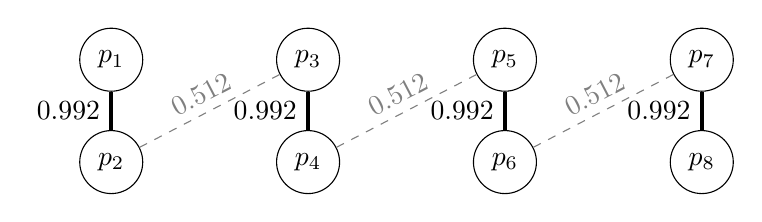
\begin{tikzpicture}[
    processo/.style={circle,draw,minimum size=8mm},
    forte/.style={line width=1.5pt},
    fraca/.style={dashed,gray},
    grupo/.style={draw,dashed,rounded corners,inner sep=6pt}
]
\node[processo] (p1) at (0,0) {$p_1$};
\node[processo] (p2) at (0,-1.3) {$p_2$};
\node[processo] (p3) at (2.5,0) {$p_3$};
\node[processo] (p4) at (2.5,-1.3) {$p_4$};
\node[processo] (p5) at (5,0) {$p_5$};
\node[processo] (p6) at (5,-1.3) {$p_6$};
\node[processo] (p7) at (7.5,0) {$p_7$};
\node[processo] (p8) at (7.5,-1.3) {$p_8$};

\draw[forte] (p1) -- node[left] {$0.992$} (p2);
\draw[forte] (p3) -- node[left] {$0.992$} (p4);
\draw[forte] (p5) -- node[left] {$0.992$} (p6);
\draw[forte] (p7) -- node[left] {$0.992$} (p8);

\draw[fraca] (p2) -- node[above,sloped] {$0.512$} (p3);
\draw[fraca] (p4) -- node[above,sloped] {$0.512$} (p5);
\draw[fraca] (p6) -- node[above,sloped] {$0.512$} (p7);
\end{tikzpicture}
\caption{Representação simplificada do grafo de afinidade. Algumas ligações foram omitidas para facilitar a leitura.}
\label{fig:grafo-afinidade-exemplo}
\end{figure}

O \textit{spectral clustering} analisa o grafo de afinidade para
identificar processos fortemente relacionados. Os processos são depois
separados em $B=4$ clusters através do K-Means.

Para o exemplo considerado, são obtidos os seguintes \textit{bundles}:

\begin{equation}
\begin{aligned}
    B_0 = \{p_1,p_2\}, &
    B_1 &= \{p_3,p_4\},\\
    B_2 &= \{p_5,p_6\}, &
    B_3 &= \{p_7,p_8\}.
\end{aligned}
\end{equation}

As cargas agregadas resultantes são:

\begin{table}[H]
\centering
\begin{tabular}{|c|c|c|c|}
\hline
\textbf{Bundle} & \textbf{Processos} &
\textbf{$W_b$} & \textbf{$R_b$ (MB)} \\
\hline
$B_0$ & $p_1,p_2$ & $0.10+0.11=0.21$ & $210$ \\
$B_1$ & $p_3,p_4$ & $0.20+0.21=0.41$ & $410$ \\
$B_2$ & $p_5,p_6$ & $0.30+0.31=0.61$ & $610$ \\
$B_3$ & $p_7,p_8$ & $0.40+0.41=0.81$ & $810$ \\
\hline
\end{tabular}
\caption{Bundles e respetivas grandezas agregadas.}
\label{tab:exemplo-bundles-formados}
\end{table}

Nenhum destes \textit{bundles} requer divisão adicional, uma vez que os
seus processos apresentam cargas semelhantes e os valores agregados não
excedem os limites de qualidade considerados.

A partir deste ponto, cada \textit{bundle} passa a ser tratado como uma
entidade individual. Assim, o QUBO global possui

\begin{equation}
    N K = 4 \times 2 = 8
\end{equation}

variáveis binárias.
